\documentclass[10pt,presentation]{beamer}

%%%%%%%%%%%%%%%%%%%%%%%%%%%%%%%%%%%%%
%% Select input file encoding:
%%   utf8   - UTF-8, nowadays standard on most operating systems
%%   latin1 - ISO-8859-1
\usepackage[utf8]{inputenc}

%%%%%%%%%%%%%%%%%%%%%%%%%%%%%%%%%%%%%
%% Select language
%%
\usepackage[ngerman]{babel}        % Deutsch, neue Rechtschreibung
%\usepackage[english]{babel}       % English

\usetheme{rwth}
\usepackage[T1]{fontenc}           % Font encoding (don't change!)
\usepackage{lmodern}               % Select Linux Modern Fonts (don't change)
\usepackage{sansmathfonts}         % Sans fonts in math environments
\usepackage{textcomp}              % fix 'missing font symbols' warning
\renewcommand{\rmdefault}{phv}     % Arial like (Helvetica)
\renewcommand{\sfdefault}{phv}     % Arial like (Helvetica)

%% graphics related packages
\usepackage{graphicx}              % needed to include graphics (don't change)
\usepackage{epstopdf}              % required to include eps files
%\usepackage{svg}                   % include svg files (requires Inkscape)
\usepackage[encoding,filenameencoding=utf8]{grffile} % allow utf8 file names in graphics

%%%%%%%%%%%%%%%%%%%%%%%%%%%%%%%%%%%%%
%% import packages for content
%%
\usepackage{listings}                           % for lstlisting and \lstinline|..|
%% TikZ can be used to /program/ graphics.
\usepackage{tikz}                                % comment-out, if you don't need this.
%% some TikZ-libraries and settings for the examples...
\usetikzlibrary{shadings}           % GW: color gradients
\usetikzlibrary{arrows,calc,positioning,fit,matrix,shadows,chains,arrows,shapes,spy,fadings}
\usepackage{pgfplots}
\usetikzlibrary{pgfplots.units,shapes.symbols,shapes.arrows}
%\usetikzlibrary{pgfplots.external}
%\tikzexternalize[prefix=tmp/]

%% Custom packages and definitions

% Mathematikumgebung
\usepackage{amsmath}
\usepackage{amssymb}
\usepackage{sansmath}

% tabularx -> bessere "tabular"-Umgebung
\usepackage{tabularx}

% zusätzliche Formatbezeichner für die tabularx-Umgebung
\newcolumntype{L}{>{\raggedright\let\newline\\\arraybackslash\hspace{0pt}}X}
\newcolumntype{R}{>{\raggedleft\let\newline\\\arraybackslash\hspace{0pt}}X}
\newcolumntype{C}{>{\centering\let\newline\\\arraybackslash\hspace{0pt}}X}

% center text vertically in tabularx(column)
%\renewcommand{\tabularxcolumn}[1]{>{\large}m{#1}}

% Bessere Tabellenlinien
\usepackage{booktabs}

% Tabellenzeilen für booktabs anpassen -> call on frame with table
\newcommand{\fixbooktabsrowhight}{%
    \setlength{\aboverulesep}{0pt}
    \setlength{\belowrulesep}{0pt}
    \setlength{\extrarowheight}{.5ex}
}

% Zellen über mehrere Zeilen
\usepackage{multirow}

% Source, e.g. for images
\setbeamercolor{framesource}{fg=gray}
\setbeamerfont{framesource}{size=\tiny}

\usepackage[absolute,overlay]{textpos}
\newcommand{\source}[1]{\begin{textblock*}{\linewidth}(1ex,\paperheight-2.75em)
        \begin{beamercolorbox}[left]{framesource}
            \usebeamerfont{framesource}\usebeamercolor[fg]{framesource} Source: {#1}
        \end{beamercolorbox}
\end{textblock*}}

\usepackage{etoolbox}
%% short titles for toc \(sub)section[SHORTTITLE for toc]{LONGTITLE for slide}
\makeatletter
% Insert [short title] for \section in ToC
\patchcmd{\beamer@section}{{#2}{\the\c@page}}{{#1}{\the\c@page}}{}{}
% Insert [short title] for \section in Navigation
\patchcmd{\beamer@section}{{\the\c@section}{\secname}}{{\the\c@section}{#1}}{}{}
% Insert [short title] for \subsection in ToC
\patchcmd{\beamer@subsection}{{#2}{\the\c@page}}{{#1}{\the\c@page}}{}{}
% Insert [short title] for \subsection  in Navigation
\patchcmd{\beamer@subsection}{{\the\c@subsection}{#2}}{{\the\c@subsection}{#1}}{}{}
\makeatother

%% MEF packages and commands
\usepackage{multicol}
\usepackage[version=3]{mhchem} % Formula subscripts using \ce{}
\newcommand{\nox}{NO$_x$} % our abbreviation
\usepackage{subfigure}
\usepackage{scrextend} %needed for footnotes in tables
\DeclareRobustCommand{\ILS}{
\includegraphics[height=\fontcharht\font`T]{/home/fuller/Dropbox/Documents/TeX/ILS_bold}}

%get proper bib with numbered entries
\setbeamertemplate{bibliography item}{\insertbiblabel}

%footnote citations - replace \cite with \footcite or \footfullcite
\usepackage[backend=bibtex, style=chem-acs]{biblatex} %, style=authoryear-comp
\addbibresource{/home/fuller/Dropbox/Documents/TeX/bibfiles/references}
\addbibresource{/home/fuller/Dropbox/Documents/TeX/bibfiles/ownpubspres}

%shrink citations
\setbeamerfont{footnote}{size=\tiny}

%no ``figure'' in caption
\setbeamertemplate{caption}{\insertcaption} 

\newcommand{\red}[1]{\textcolor{red}{#1}} %easy red text
\usepackage{ulem}
\newcommand{\soutthick}[1]{%
	\renewcommand{\ULthickness}{1.6pt}%
	\sout{#1}%
	\renewcommand{\ULthickness}{.4pt}% Resetting to ulem default
}

%add YAML to listings: https://www.latex4technics.com/?note=187E
\newcommand\YAMLcolonstyle{\color{red}\mdseries}
\newcommand\YAMLkeystyle{\color{black}\bfseries}
\newcommand\YAMLvaluestyle{\color{blue}\mdseries}

\makeatletter

% here is a macro expanding to the name of the language
% (handy if you decide to change it further down the road)
\newcommand\language@yaml{yaml}

\expandafter\expandafter\expandafter\lstdefinelanguage
\expandafter{\language@yaml}
{
	keywords={true,false,null,y,n},
	keywordstyle=\color{darkgray}\bfseries,
	basicstyle=\YAMLkeystyle,                                 % assuming a key comes first
	sensitive=false,
	comment=[l]{\#},
	morecomment=[s]{/*}{*/},
	commentstyle=\color{purple}\ttfamily,
	stringstyle=\YAMLvaluestyle\ttfamily,
	moredelim=[l][\color{orange}]{\&},
	moredelim=[l][\color{magenta}]{*},
	moredelim=**[il][\YAMLcolonstyle{:}\YAMLvaluestyle]{:},   % switch to value style at :
	morestring=[b]',
	morestring=[b]",
	literate =    {---}{{\ProcessThreeDashes}}3
	{>}{{\textcolor{red}\textgreater}}1     
	{|}{{\textcolor{red}\textbar}}1 
	{\ -\ }{{\mdseries\ -\ }}3,
}

% switch to key style at EOL
\lst@AddToHook{EveryLine}{\ifx\lst@language\language@yaml\YAMLkeystyle\fi}
\makeatother

\newcommand\ProcessThreeDashes{\llap{\color{cyan}\mdseries-{-}-}}



\title{Progress in \soutthick{ Nitrogen } Novel Combustion Chemistry}
%\subtitle{Subtitle}
%\titlegraphic{}
\author{Mark E. Fuller, Ph.D.}
\email{fuller@pcfc.rwth-aachen.de} % optionally
\institute{Physico-Chemical Fundamentals of Combustion}
%\webaddress{www.informatik.rwth-aachen.de/mentoring} % overrides www.rwth-aachen.de
\date{\today}
\subject{RWTH presentation template}
\keywords{RWTH, Latex Beamer, template}

%\logo{\includegraphics[height=8mm]{logos/logo}} % will replace the default logo

% official institute logo offset correction
%\logo{\vskip-3.5mm\includegraphics[height=12.5mm]{logos/rwth_mentoring_rgb.eps}\hspace{-2mm}} % optionally
\logo{\vskip-2mm
\includegraphics[width=45mm]{logos/PCFC.png}\hspace{-2mm}} % optionally

% alternative logo position (not recommended)
%\instlogo{\includegraphics[height=10mm]{logos/rwth_mentoring_rgb.eps}} % optionally

%%%%%%%%%%%%%%%%%%%%%%%%%%%%%%%%%%%%%
%% configure template behaviour
%%-------------------------------
%%   secstart -- style of section start
%%               selectable parameters:
%%                 sectitle:  only provides section title
%%                 sectoc:    display section table of contents
%%                 <empty>:   display nothing on section start
\secstart{sectitle}
% disable PDF navigation icons
\setbeamertemplate{navigation symbols}{}

\begin{document}
    
\begin{frame}{\nox\ interactions in hydrocarbon combustion}
    \begin{figure}
        \centering
        \includegraphics[width=0.8\linewidth]{NOx_Cycle.png}
        \caption{And when \ce{RH} is replaced with \ce{QOOH} or \ce{OOQOOH}?}
        \label{fig:NOx_cycle}
    \end{figure}
\end{frame}

\begin{frame}{Key sources}
    \begin{itemize}
        \item Bugler {\it et al.}\footfullcite{Bugler.2016} mechanism for pentane combustion
        \item Nitrogen combustion chemistry of Glarborg {\it et al.}\footfullcite{Glarborg.2018} (maximum two carbon atoms)
        \item Pathways and classes of reactions between {\it n}-pentane and \nox\ from Marrod\'an {\it et al.}\footfullcite{Marrodan.2019}
    \end{itemize}
\end{frame}

\begin{frame}{Latest revisions}
    \begin{itemize}
        \item The \ce{HNO2} potential energy surface (PES) reactions calculated by Chen {\it et al.}\footfullcite{Chen.2019}
        \item Rates for the \ce{H2NO2} and \ce{CH4NO2} PES from Fuller and Goldsmith\footfullcite{Fuller.2018}
        \item Hydrogen abstraction by \ce{NO2} from alkanes and alkenes as published by Chai and Goldsmith\footfullcite{Chai.2017} and refit to the exothermic direction\footfullcite{Fuller.2018, Fuller.2020}
        \item Decomposition rates for nitromethane (and related reactions)\footfullcite{Annesley.2015}, alkyl nitrites\footfullcite{Randazzo.2018}, and isopropyl nitrate\footfullcite{Fuller.2019.A}
        \item The \ce{C3H3NO} PES as calculated by Danilack and Goldsmith\footfullcite{Danilack.2018}
    \end{itemize}
\end{frame}

\begin{frame}{Reaction Classes and Examples}
    Develop mechanism by systematic inclusion of reaction classes
    \begin{itemize}
        \item Hydrogen abstractions by \nox to form \ce{HONO}, \ce{HNO2}, \ce{HNO}
        \item Unimolecular conformer formation and dissociation
        \begin{itemize}
            \item \ce{RNO2}$\rightleftharpoons$ \ce{R} + \ce{NO2}
            \item \ce{RONO}$\rightleftharpoons$ \ce{RO} + \ce{NO}
            \item \ce{RONO2}$\rightleftharpoons$ \ce{RO} + \ce{NO2}
        \end{itemize}
        \item Isomerizations  
        \begin{itemize}
            \item \ce{RONO}$\rightleftharpoons$ \ce{RNO2}
        \end{itemize}
        \item Concerted \ce{HONO} elimination
        \begin{itemize}
            \item \ce{RONO}$\rightleftharpoons$ alkene + \ce{HONO}
        \end{itemize}
        \item \nox\ cycling reactions
        \begin{itemize}
            \item \ce{RO2} + \ce{NO} $\rightleftharpoons$ \ce{RO} + \ce{NO2}
            \item \ce{RO} + \ce{NO} $\rightleftharpoons$ \ce{R} + \ce{NO2}
        \end{itemize}
    \end{itemize}
\end{frame}


\begin{frame}{Experimental impact of \nox on {\it n}-pentane ignition delay times}
\begin{figure}
	\centering
	\includegraphics[width=\linewidth]{/home/fuller/Dropbox/Documents/PCFC/Experimental/RCM/NOx_Project/Sim_Model/Plot_nP_NOx_phi_1_AllDope.png}
	\caption{Comparison of stoichiometric {\it n}-pentane ignition delay times; P$_C$=15 bar, mixtures in synthetic air diluted with additional nitrogen or argon as indicated.
		{\it n}-\ce{C5H12} : 8 (\ce{O2} + 3.76 \ce{N2} + 3.76 \ce{X}) where X is either \ce{N2} or \ce{Ar}.
		Open symbols are experiments conducted with \ce{N2} diluent; open symbols are \ce{Ar} diluent.
		Black circles are neat {\it n}-pentane.
		Red squares are 333 ppm \ce{NO2} dopant.
		Blue triangles are 1000 ppm \ce{NO} dopant.}
	\label{fig:phi1comp}
\end{figure}
\end{frame}

\begin{frame}{The old (slow) way forward}
	\begin{multicols}{2}
	\begin{enumerate}
		\item Calculate sensitivities
		\item Tweak/add some rates*
		\item Run simulations
		\item Feel sad and start over
	\end{enumerate}
	\columnbreak
	\centering
	{\scriptsize *Until this...\\}
	\vspace{0.1cm}
	\includegraphics[width=0.8\columnwidth]{NOx_Cycle.png}
	\vspace{0.1cm}
	{\scriptsize ...becomes this (or worse!)}
	\vspace{0.1cm}
	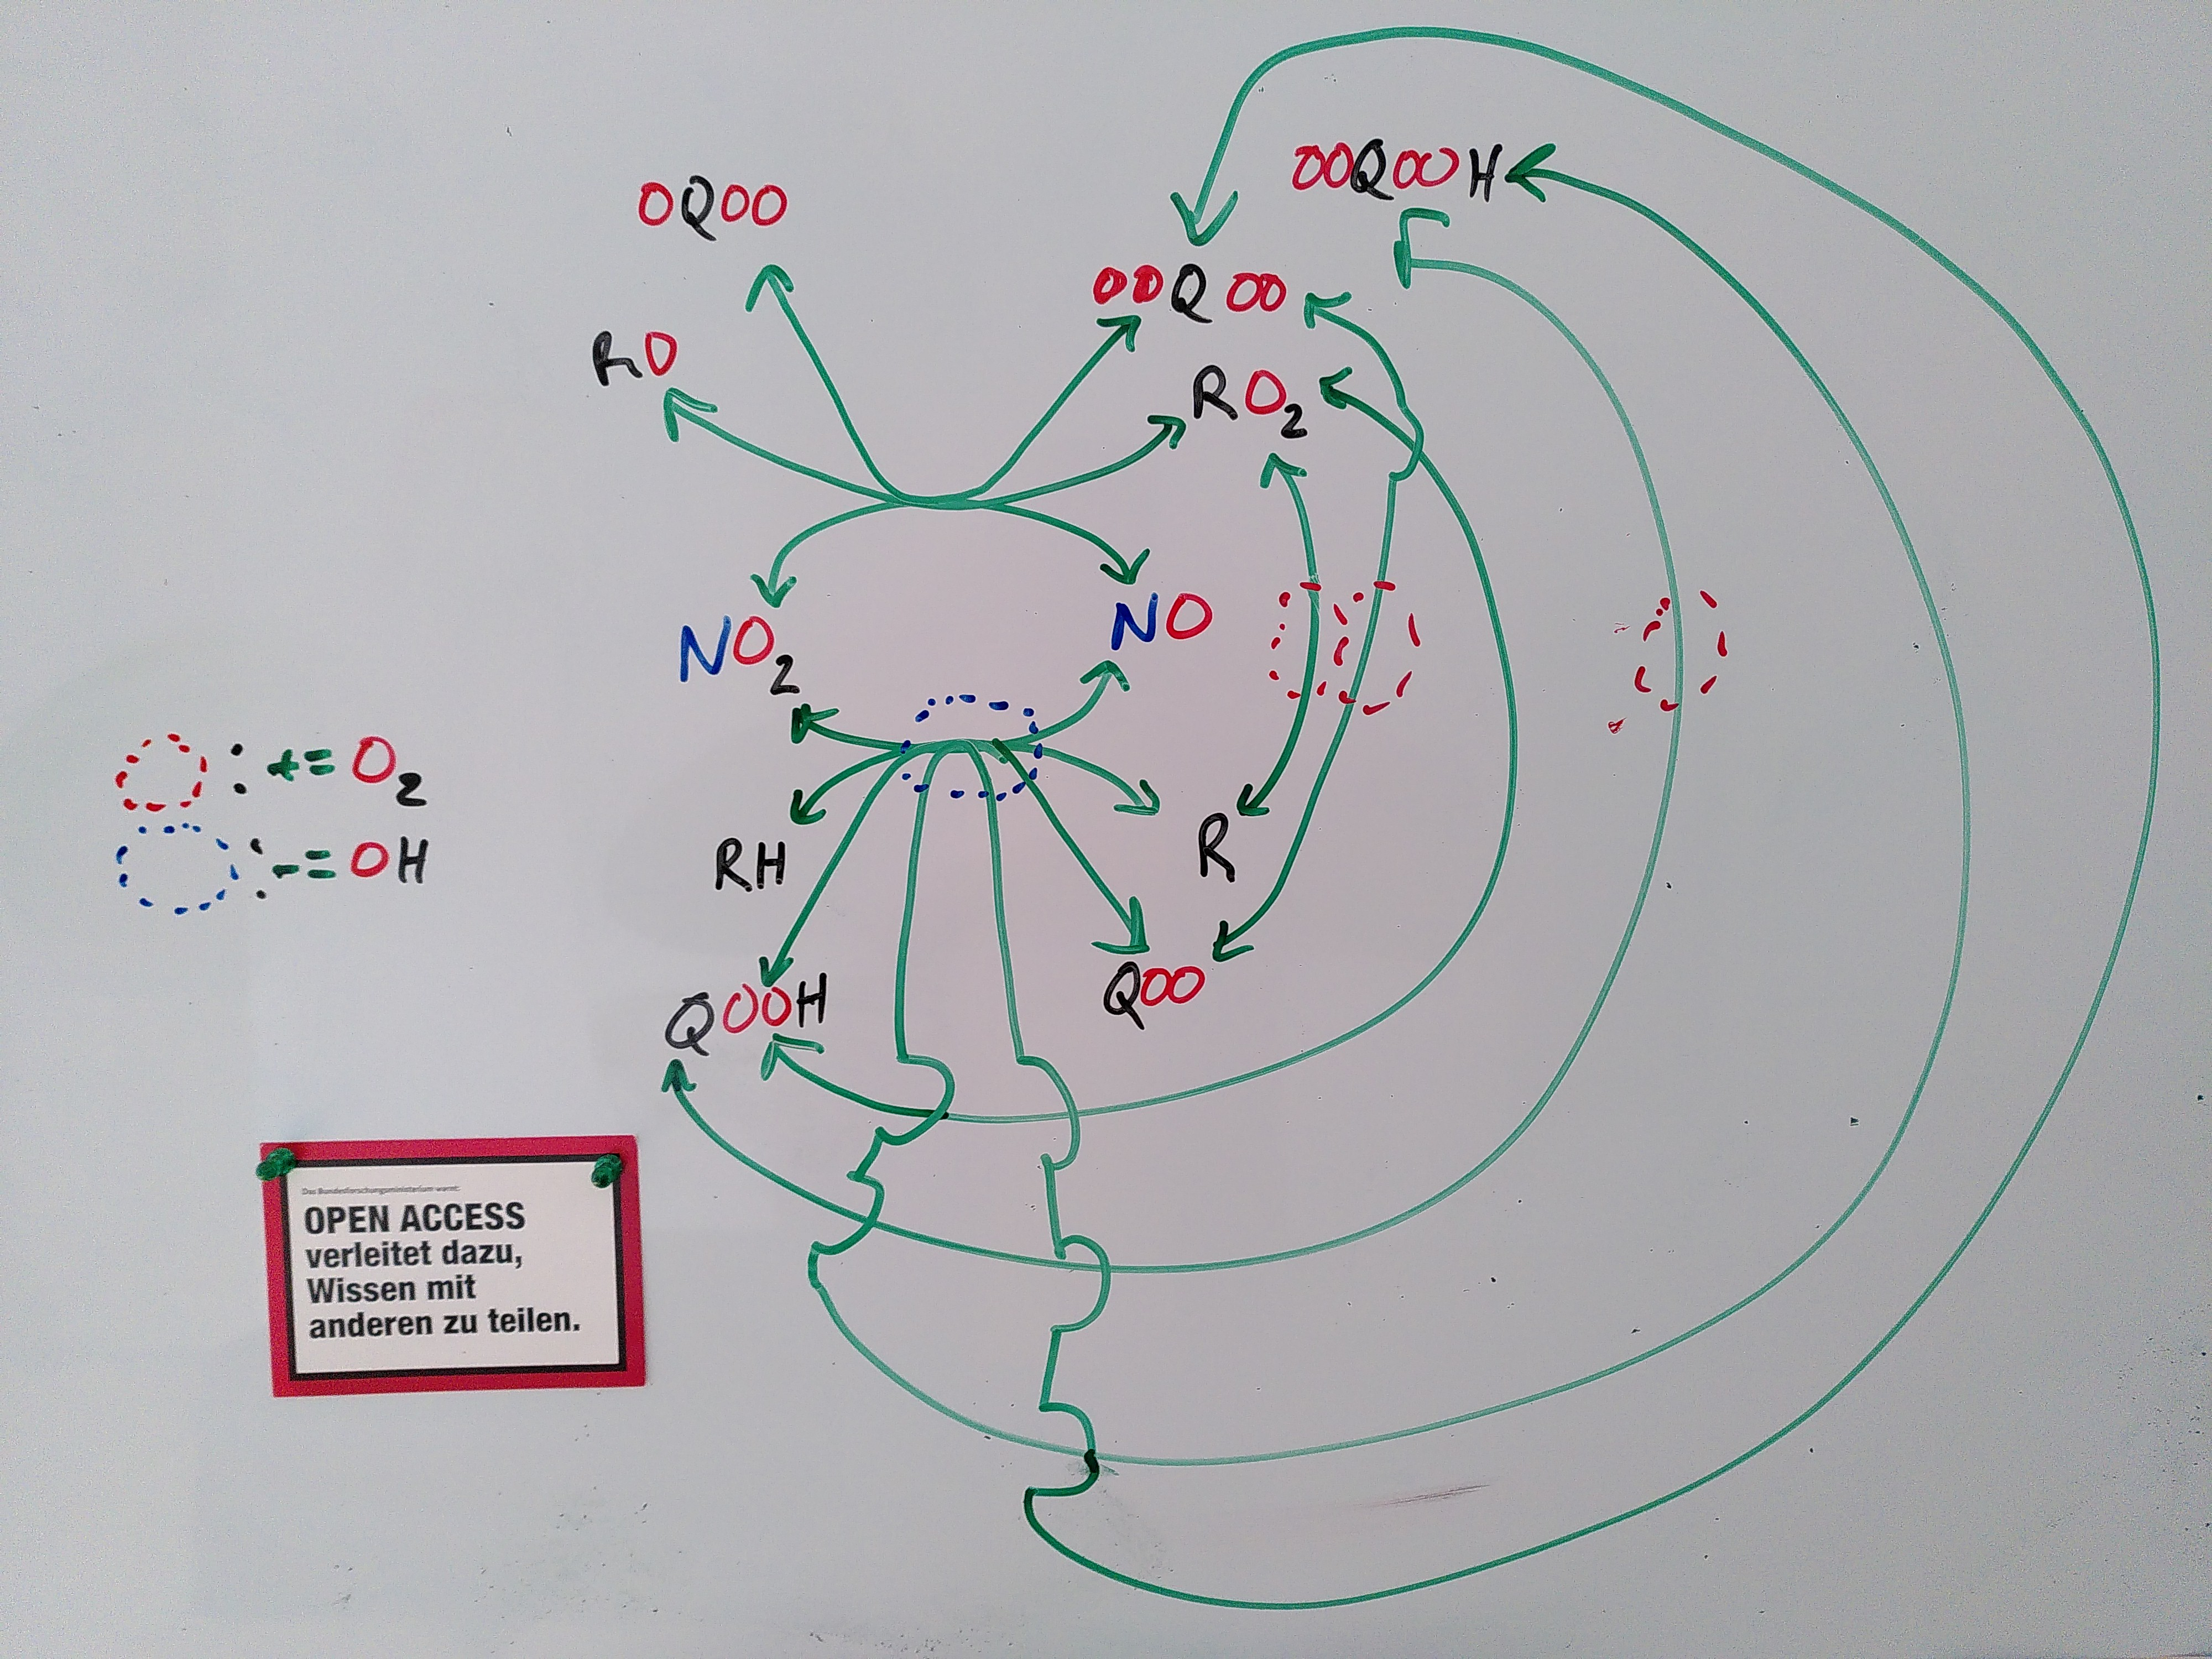
\includegraphics[width=0.8\columnwidth]{BigNOxCycle.jpg}
	\end{multicols}
\end{frame}

\begin{frame}{Model predictions}    
    \begin{figure}
    	\centering
    	\begin{tabular}{cc}
    		\subfigure[$\phi$ = 1.0; 1000 ppm \ce{NO}; simulated $T_C$ is corrected to experimental values]{\includegraphics[width=0.45\linewidth]{/home/fuller/Dropbox/Documents/PCFC/Experimental/RCM/NOx_Project/Sim_Model/Plot_nP_NOx_phi_1_dope_1e3NO-correctedT.png}} &
    		
    		\subfigure[$\phi$ = 1.0; 333 ppm \ce{NO2}]{\includegraphics[width=0.45\linewidth]{/home/fuller/Dropbox/Documents/PCFC/Experimental/RCM/NOx_Project/Sim_Model/Plot_nP_NOx_phi_1_dope_333NO2.png}}
        \end{tabular}
    	\caption{The solid blue line is the original model presented in this work and the dashed yellow line is the optimized version with improved rate rules.
    	The green dash-dot line is the original model with the \ce{OOQOOH} + \ce{NO} reactions of Marrod\'an {\it et al.}.
    	The red dotted line in the model of Marrod\'an {\it et al.}}
    \end{figure}
\end{frame}

\begin{frame}{Sensitivities}
    \begin{figure}
        \centering
        \begin{tabular}{cc}
            \subfigure[$\phi$ = 1.0; 1000 ppm \ce{NO}]{\includegraphics[width=0.45\linewidth]{../SACVS/SensPlot_MEF_0_NO_phi_1_0.png}} &
            
            \subfigure[$\phi$ = 1.0; 333 ppm \ce{NO2}]{\includegraphics[width=0.45\linewidth]{../SACVS/SensPlot_MEF_0_NO2_phi_1_0.png}}
        \end{tabular}
    \end{figure}
\centering
The sensitive rates are hard or impossible to access by experiment! So we calculate or estimate.
\end{frame}     

\begin{frame}{Problem: Calculations are expensive}
	\begin{figure}
		\centering
		\includegraphics[width=0.8\columnwidth]{PES_2-pentyl_no2_1.pdf}
		\caption{Potential energy surface for the 2-pentyl + \ce{NO2} system. Energies in kcal/mol.
			With all the time required for restarting jobs, tweaking scans, etc., this is tedious}
		\label{fig:2-pentyl_PES}
	\end{figure}
\end{frame}

\begin{frame}{Progress on \nox-Cycling}
	\begin{figure}
		\centering
		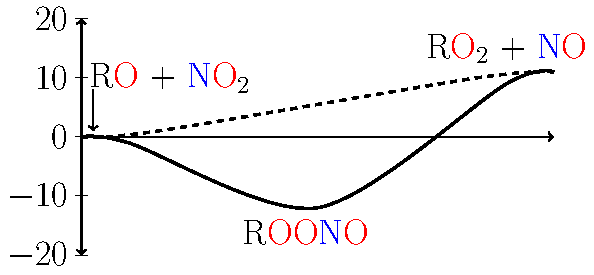
\includegraphics[width=0.5\columnwidth]{PES_NOx-Cycle.pdf}
		\caption{Generalized potential energy surface for alkoxy radical (RO) + \ce{NO2} system. Energies in kcal/mol.
			Well-skipping occurs at virtually all combustion-relevant temperatures and pressures.}
		\label{fig:NOx-Cycle_PES}
	\end{figure}
\begin{tabular}{crrr}
	\toprule
	Reaction & \multicolumn{1}{c}{$A$} & \multicolumn{1}{c}{$n$} & \multicolumn{1}{c}{$E_a$}\\
	\midrule
	\ce{CH3O2} + \ce{NO} $\rightleftharpoons$ \ce{CH3O} + \ce{NO2} & 4.62E+15 & -0.38 & 97.8\\
	\ce{C2H5O2} + \ce{NO} $\rightleftharpoons$ \ce{C2H5O} + \ce{NO2} & 2.11E+14 & -0.12 & -470.6\\
	\ce{NC3H7O2} + \ce{NO} $\rightleftharpoons$ \ce{NC3H7O} + \ce{NO2} & 1.07E+14 & -0.25 & -1302.0\\

	\bottomrule
\end{tabular}	

Units: centimeters, kelvin, calories, moles
\end{frame}

\begin{frame}{Problem: Refining rates has to be done intelligently}
	\begin{figure}
		\centering
		\begin{tabular}{ccc}
			\subfigure[\scriptsize \ce{HNO} + \ce{NO2} $\rightleftharpoons$ \ce{HNO2} + \ce{NO}]{\includegraphics[width=0.3\linewidth]{../Optimization/CompOptRate_1_4202.png}\label{fig:NOxCycle-0}} &
			
			\subfigure[\scriptsize \ce{C2H5O2} + \ce{NO} $\rightleftharpoons$ \ce{C2H5O} + \ce{NO2}]{\includegraphics[width=0.3\linewidth]{../Optimization/CompOptRate_2_4203.png}\label{fig:NOxCycle-C2}} 
			
			\subfigure[\scriptsize \ce{RO2} + \ce{NO} $\rightleftharpoons$ \ce{ROONO} ]{\includegraphics[width=0.3\linewidth]{../Optimization/CompOptRate_33_4171.png}\label{fig:NOxCycleWell-NO}} 
		\end{tabular}
		\caption{Comparison of estimated and optimized rates for selected \nox-cycling reactions.
			Sure these fits are ``optimized", but they're dumb - human intervention or better (more) validation data is required!}
	\end{figure}
\end{frame}  

\begin{frame}{(Sort of) Good news: People are working on this and have tools we can try!}
	\begin{figure}
		\centering
		\includegraphics[width=0.75\columnwidth]{Frhodo.png}
		\caption{Travis Sikes' and Rob Tranter's Frhodo for laser schlieren, isobaric, and isochoric reactors}
	\end{figure}
	%User-friendly integrated manual and automated adjustment of rates (in development)\footnote{ \url{https://github.com/Argonne-National-Laboratory/Frhodo}}
\end{frame}

\begin{frame}{Intermission}
	\centering
	{\huge There are big(ger)-picture questions we need to ask about our research processes, particularly for novel chemistry and compounds ({\it e.g.} sulfur, nitrogen, halogens)}
\end{frame}

\begin{frame}{What does publishing all of these (highly-empirical) models get us?}
	\begin{enumerate}
		\item Of course we need data (our current publications)
		\item We also need rules and analogies to guess rates
		\item Then we need good methods for refining rates and/or calculating better estimates
		\item And we need (human and machine) readable databases of validation targets
	\end{enumerate}
\end{frame}                 

\begin{frame}{What does publishing all of these (highly-empirical) models get us?}
	\begin{figure}
		\centering
		\includegraphics[width=0.8\columnwidth]{profzi.png}
		\caption{Are our epistemological models rafts or pyramids?}
	\end{figure}
\end{frame}

\begin{frame}{How do we know if we're building on sand? Validation targets are a mess}
	\begin{itemize}
		\item Getting experimental data for comparison now: spreadsheets, text files, PDFs(!), digitizing plots... Virtually no standards and usually not (easily) machine readable
		\item Some attempts have been made, but without community buy-in (and funding: €, \$, \ILS\ ), these projects stall and/or we go from $n$ different formats to $n+1$
		\item We need to motivate standardization - provide formats to store data and tools to read it back in for manipulation and analysis
		\item Compatibility with community standards and ease-of-maintenance favors open-source solutions
	\end{itemize}
\end{frame}  

\begin{frame}{Mechanism Generation: Could there be a better way?}
\begin{figure}
	\centering
	\includegraphics[width=0.8\columnwidth]{T3-circle.png}
\end{figure}
Toolchain in development under leadership of Green Group (MIT) and database under Dana Group (Technion)
\end{frame}       
%
\begin{frame}{Data Archiving and Experimental Validation: Could there be a better way?}
	\begin{multicols}{2}
	\begin{figure}
		\centering
		\includegraphics[width=\columnwidth]{pyked-logo.png}
	\end{figure}
	\columnbreak
Kyle Niemeyer and Bryan Weber have proposed the \textsc{PyKED} tools\footfullcite{PyKED} and \textsc{ChemKED} format/database\footnote{\url{https://github.com/pr-omethe-us/ChemKED-database}}.\\
\vspace{0.3cm}
The package and database are currently ``stale,'' but is being reactivated and I will be publishing my experimental data in the \textsc{ChemKED} format.\\
\vspace{0.3cm}
If would be great if PCFC could also publish and convert archived data for easy (re)use and manipulation - I want to work on this!
	\end{multicols}
\end{frame} 

\begin{frame}{Cui bono? And is it worth the effort?}
	\vspace{-0.6cm}
\begin{multicols}{2}
	\begin{itemize}
		\item I've made it dead simple (with instructions) and fast to process PCFC RCM data into \textsc{ChemKED}
		\item Instead of submitting all the files with the manuscript, a directory is uploaded to a public repository (which is in the Arctic Code Vault!)
		\item Validation data will be in a standard place and standard format, not lost of one of our machines (good luck with the move to SWL!).
		\item Open formats and software will minimize in-house efforts (Philipp's toolbox?)
	\end{itemize}
\columnbreak
{\tiny
	\ldots
\lstinputlisting[language=YAML,firstline=9,lastline=18]{/home/fuller/Dokumente/PCFC/Model/c5-n-mechanism-development/publication/supplemental/SimFile_250_CK.yaml}
	\ldots
\lstinputlisting[language=YAML,firstline=63,lastline=80]{/home/fuller/Dokumente/PCFC/Model/c5-n-mechanism-development/publication/supplemental/SimFile_250_CK.yaml}
	\ldots}
\end{multicols}
\end{frame}

\begin{frame}{And who will maintain and develop \textsc{PyKED}?}
	\begin{multicols}{2}
		\begin{figure}
			\centering
			\includegraphics[height=2in]{/home/fuller/Bilder/Alon_3_small.jpg}
		\end{figure}
	\centering
	Prof. Alon Grinberg Dana (Head, Dana Research Group, Technion)
		\columnbreak
		\begin{figure}
			\centering
			\includegraphics[height=2in]{/home/fuller/Bilder/Profile/Fuller_RWTH_3.jpg}
		\end{figure}
	\centering
	 Dana Group Lab Manager (starting Fall 2021)
	\end{multicols}
%\centering
%Experiments beginning Fall 2021 at the Technion (Haifa, Israel)
\end{frame}

\begin{frame}{Final Thoughts}
	\begin{itemize}
		\item We are in the midst of a paradigmatic shift in terms of computing and networking resources
		\item Adoption of open standards, methodologies, and software is essential for building processes to generate, analyze, and validate predictive chemical mechanisms, particularly for novel compositions and constituents

		\item The \textsc{Active Thermochemical Tables} already provide an example of accepted, benchmark, ``bulletproof'' data that has emerged from the application of such methods
		
		\item Tangentially (and even farther out), continued development of open community resources and tools can help lead us away from current problems with for-profit journals and publishing by creating avenues with improved access to source material and transparent review and validation
	\end{itemize}
\end{frame} 

\begin{frame}
	\centering
	BACKUP SLIDES
\end{frame}

\begin{frame}{Model predictions}    
	\begin{figure}
		\centering
		\begin{tabular}{cc}    		
			\subfigure[$\phi$ = 0.5; 1000 ppm \ce{NO}]{\includegraphics[width=0.45\linewidth]{/home/fuller/Dropbox/Documents/PCFC/Experimental/RCM/NOx_Project/Sim_Model/Plot_nP_NOx_phi_05_dope_1e3NO.png}} &
			
			\subfigure[$\phi$ = 0.5; 333 ppm \ce{NO2}]{\includegraphics[width=0.45\linewidth]{/home/fuller/Dropbox/Documents/PCFC/Experimental/RCM/NOx_Project/Sim_Model/Plot_nP_NOx_phi_05_dope_333NO2.png}}
		\end{tabular}
		%        \caption{The solid blue line is the original model presented in this work and the dashed yellow line is the optimized version with improved rate rules.
		%    	The green dash-dot line is the original model with the \ce{OOQOOH} + \ce{NO} reactions of Marrod\'an {\it et al.}.
		%    	The red dotted line in the model of Marrod\'an {\it et al.}}
	\end{figure}
\end{frame}
%
\begin{frame}{Model predictions}    
	\begin{figure}
		\centering
		\begin{tabular}{cc}    		
			\subfigure[$\phi$ = 2.0; 1000 ppm \ce{NO}]{\includegraphics[width=0.45\linewidth]{/home/fuller/Dropbox/Documents/PCFC/Experimental/RCM/NOx_Project/Sim_Model/Plot_nP_NOx_phi_2_dope_1e3NO.png}} &
			
			\subfigure[$\phi$ = 2.0; 333 ppm \ce{NO2}]{\includegraphics[width=0.45\linewidth]{/home/fuller/Dropbox/Documents/PCFC/Experimental/RCM/NOx_Project/Sim_Model/Plot_nP_NOx_phi_2_dope_333NO2.png}} 
		\end{tabular}
		%        \caption{The solid blue line is the original model presented in this work and the dashed yellow line is the optimized version with improved rate rules.
		%    	The green dash-dot line is the original model with the \ce{OOQOOH} + \ce{NO} reactions of Marrod\'an {\it et al.}.
		%    	The red dotted line in the model of Marrod\'an {\it et al.}}
	\end{figure}
\end{frame}

\begin{frame}{Temperature-shift due to excessive reactivity during compression}    
	\begin{figure}
		\centering
		\begin{tabular}{cc}
			\subfigure[$\phi$ = 1.0; 1000 ppm \ce{NO}]{\includegraphics[width=0.45\linewidth]{/home/fuller/Dropbox/Documents/PCFC/Experimental/RCM/NOx_Project/Sim_Model/Plot_nP_NOx_phi_1_dope_1e3NO.png}} &
			
			\subfigure[$\phi$ = 1.0; 1000 ppm \ce{NO}; simulated $T_C$ is corrected to experimental values]{\includegraphics[width=0.45\linewidth]{/home/fuller/Dropbox/Documents/PCFC/Experimental/RCM/NOx_Project/Sim_Model/Plot_nP_NOx_phi_1_dope_1e3NO-correctedT.png}}
		\end{tabular}
	\end{figure}
\end{frame}  

\end{document}